\documentclass[a4paper, oneside]{csthesis}

\usepackage{etex}
\reserveinserts{28}

% package to be able to use special characters
\usepackage[utf8]{inputenc}

% Sophisticated math package
\usepackage{amsmath}

% Special symbols
\usepackage{amssymb}

\usepackage{siunitx}

% nicely render theorems and proofs
\usepackage[standard,thmmarks,amsmath]{ntheorem}

\usepackage{graphicx}

% package to format pseudo-code. Check the package documentation.
% http://ctan.org/pkg/listings
\usepackage{algorithmic}
\usepackage{algorithm}

% awesome code highlighting and coloring for many languages
% http://en.wikibooks.org/wiki/LaTeX/Packages/Listings
\usepackage{listings}
\lstset{language=Java}

% Provides \xspace command that evaluates to a space if the next character in the source is a blank and
% no space if next character is no blank. Useful in command definitions.
\usepackage{xspace}

% Provides a more flexible tabular environment
\usepackage{tabularx}

% Enables the use of the H location specifier for float environments that puts the float exactly where it is located in the source.
\usepackage{float}

% Enables the use of colours
\usepackage{color}

\usepackage{paralist}

% nice string commands
\usepackage{xstring}

\usepackage{colortbl}
\usepackage[table]{xcolor}

% wide tables
\usepackage{adjustbox}

\definecolor{DarkGray}{gray}{0.7}
\definecolor{MiddleGray}{gray}{0.8}
\definecolor{Gray}{gray}{0.9}

\definecolor{darkblue}{rgb}{0,0,.5}
% Enables clickable links in the PDF and additional PDF specific configuration options.
\usepackage[
            colorlinks=true,
            linkcolor=darkblue, urlcolor=darkblue, citecolor=darkblue,
						raiselinks=true,
            bookmarks=true,
            bookmarksopenlevel=1,
            bookmarksopen=true,
            bookmarksnumbered=true,
            hyperindex=true,
            plainpages=false,
            pdfpagelabels=true,
            pdfstartview=FitH,
            pdfstartpage=1,
            pdfpagelayout=OneColumn
            ]{hyperref}

% Provides a highly configurable way to create references inside the document and automatically prefix
% the number reference by fig./eq./chapter and so on. You only have to use \cref{label} or \Cref{label}
% to obtain "Lemma 4.1" or "Corollary 4.1" etc., depending on the label. See an example in the proof
% of the first theorem or check the documentation of the package for further information.
\usepackage[noabbrev]{cleveref}


% awesome figure placment
\usepackage{subfigure}

% Load own command definitions, a few helpful ones are already defined there.

% This alters the numbering of theorems and lemmas.
\theoremsymbol{\ensuremath{\scriptstyle \Diamond}}
\renewtheorem{theorem}{Theorem}[chapter]
\renewtheorem{lemma}[theorem]{Lemma}
\renewtheorem{corollary}[theorem]{Corollary}
\renewtheorem{definition}[theorem]{Definition}

% This creates a two new theorem-like environments
\theoremsymbol{}
\newtheorem{notation}[theorem]{Notation}
\theorembodyfont{}
\newtheorem*{problem}{Problem}

\crefname{algorithm}{algorithm}{algorithms}
\Crefname{algorithm}{Algorithm}{Algorithms}

% This changes the comment style of the "algorithmic" pseudocode package
\renewcommand\algorithmiccomment[1]{\hfill \small \(\triangleright\) #1}

% This creates four commands to leave annotations in your document
\newcommand{\TODO}[1]{\noindent {{\color{red}\fbox{\sffamily \bfseries TODO}} \sffamily #1}}
\newcommand{\FIXME}[1]{\noindent {{\color{green}\fbox{\sffamily \bfseries FIXME}} \sffamily #1}}
\newcommand{\CONSIDER}[1]{\noindent {{\color{blue}\fbox{\sffamily \bfseries CONSIDER}} \sffamily #1}}
\newcommand{\RW}[1]{\noindent \color{blue}#1}

% This creates a command to easily refer to websites as footnotes
\newcommand{\websource}[3]{\footnote{{#1\newline Available at: #2 [Accessed
#3]}}}

\newcommand\telesto{\textit{Telesto}}

\graphicspath{{figures/}}

% style whole rows in table
\usepackage{array}
\newcolumntype{$}{>{\global\let\currentrowstyle\relax}}
\newcolumntype{^}{>{\currentrowstyle}}
\newcommand{\rowstyle}[1]{\gdef\currentrowstyle{#1}%
  #1\ignorespaces
}


%%%%%%%%%%%%%%%%%%%%%%%%%%%%%%%%%%%%%%%%%%%%%%%%%%%%%%%%%%%%%%%%%%%%%%%%%%%%%%%%%%%%%%%%%%%%%%%%%
% DOCUMENT METADATA

\thesistype{Report Group 32}
\title{Analytical Queuing Model for Telesto}

\author{Dominic Langenegger}
\email{dominicl@student.ethz.ch}
\institute{Advanced Systems Lab 2013 \\[2pt]
Systems Group \\[2pt]
ETH Z\"urich}

% You can put in your own logo here "\includegraphics{...}" or just comment the command
% \logo{}

\supervisors{Markus Pilman\\[2pt] Prof.\ Dr.\ Gustavo Alonso}

% You can comment the following two commands if you don't need them
\keywords{}
%\categories{ACM categories go here.}

\date{December 20, 2013}

%%%%%%%%%%%%%%%%%%%%%%%%%%%%%%%%%%%%%%%%%%%%%%%%%%%%%%%%%%%%%%%%%%%%%%%%%%%%%%%%%%%%%%%%%%%%%%%%%

\begin{document}

\frontmatter
\maketitle % do not remove this line

\cleardoublepage

%\begin{acknowledgements}
%\end{acknowledgements}


\begin{abstract}
	This report summarizes the work of analytically modeling and evaluating
	\telesto, the Distributed Message Passing System built by Simon Marti and
	Dominic Langenegger during the first milestone of the course project of the
    {\it Advanced Systems Lab} course 2013 at ETH Zurich. All relevant
    information about the first milestone can be found in \cite{asl:telesto}.

    Used concepts, mathematical formulas and theoretical aspects are heavily
    based on \cite{jain2008art} and the lecture slides.
    
\end{abstract}

\tableofcontents

\mainmatter % do not remove this line

% Start writing here
\chapter{Analytical Queuing Model}
    This chapter introduces the analytical queuing model built to model the
    characteristics of \telesto. It also includes explanations about
    simplifications and assumptions that were made.

    We recall Table 5.3 in \cite{asl:telesto}, showing in which parts of the
    system a request spends how much time. \Cref{tbl:time-middleware} shows very
    similar data (taken from an other experiment) and includes dispatching time. 
    
    \begin{table}[hp]
        \centering
        \rowcolors{1}{Gray}{white}
        \begin{tabular}{$l^c^r}
            \rowcolor{DarkGray}
            \rowstyle{\bfseries}
            Phase & Time & Relative\\
            \hline
            Dispatching & \SI{12}{\micro\second} & 0.14\%\\
            Parsing request & \SI{14}{\micro\second} & 0.17\%\\    
            Waiting for database & \SI{8,059}{\micro\second} & 99.40\%\\
            Responding & \SI{22}{\micro\second} & 0.27\%\\       
        \end{tabular}
        \caption{Time spent on various tasks by middleware workers}
        \label{tbl:time-middleware}
    \end{table}
    
    Based on this data we can safely say, that the time a request is handled by
    the middleware is minimal in comparison to the time spent to actually handle
    it on the database tier. But still we know, that the tasks the worker
    threads fullfil is also load dependent and should be modeled too.
    
    \Cref{fig:globalModel} shows the network model of \telesto{} including all
    important parts. As explained below, the clients themself are not modeled as
    separate delay centers but directly influence the network think time $z$.

    \begin{figure}[t]
        \centering
            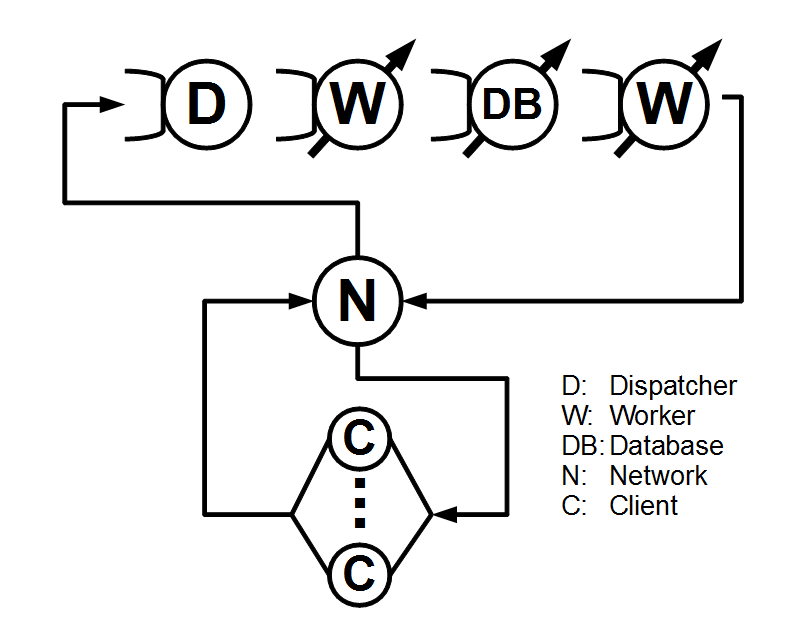
\includegraphics[width=0.9\textwidth]{model}
            \caption{Network model of the closed queuing system for \telesto}
            \label{fig:globalModel}
    \end{figure}

\section{Workload \& Model}
    As seen in \cref{fig:globalModel}, we use a closed queuing network to model
    \telesto. Since all conducted tests during milestone 1
    (see~\cite{asl:telesto} for more details) operate with clients that only
    send new requests as soon as a previous on is completed, the number of jobs
    in the system at any time is directly corresponding to the number of clients
    and therefore fixed.
    
    It is important to note, that some clients may query the middleware to
    retrieve a message when actually no message is waiting for them. Based on
    the experiments from milestone 1, we know that this is the case for roughly
    one sixth of all message requests. Notice also, that the network is only a
    delay center and therefore does not have a queue in the figure.

\subsection{Clients}
    Our queuing network does not include any modeling of the clients. This is
    because the time a job actually spends at the client is minimal since a
    client has only the following very simple tasks (that take almost no time):
    
    \begin{enumerate}[(a)]
        \item Send a message to a middleware
        \item Wait for a message
        \item Receive the message
        \item Start from (a); possibly using some information of the received
        message
    \end{enumerate}

    The actual time a job is being processed at the client is in steps (c), (d)
    and (a), which is comparable in workload to the tasks of the middleware for
    message processing as seen in~\cref{tbl:time-middleware}, excluding the part
    where the middleware waits for the database. Since this takes very little time 
    compared to the time spent processing a job at the database, it is save to 
    simplify the model by not modeling the clients as separate load
    centers.
    
    However the think time of the network can be determined by including the
    client retry delay of $100$ ms into the calculation. If we assume that (as
    stated above) roughly one sixth of all client queries end up with no message
    as a result (and therefore the clients waits those $100$ ms), we get a think
    time $T$ of about $\frac{100ms}{6} \approx 17 ms$.

\subsection{Network}
    In \telesto each client request actually passes the network in four different 
    phases:

    \begin{enumerate}
        \item Client $\rightarrow$ Middleware
        \item Middleware $\rightarrow$ Database
        \item Database $\rightarrow$ Middleware
        \item Middleware $\rightarrow$ Client
    \end{enumerate}

    Since we cannot measure the time spent in the network for the connections to
    the database individually, we don't model the network in between the
    middleware and the database separately.

    For the connection from the clients to the middlewares we can assume that
    all messages have about the same size since all conducted tests use messages
    that are never longer than about $10$ characters. This means, that we can
    assume the network delay is constant for every phase and not load dependent.
    Therefore it can simply be modeled as a delay center in the network model.

\subsection{Middleware}
    The middleware consists of a single dispatcher thread that handles all
    incoming connections and puts incoming data into a queue. This can be
    modeled as a simple fixed-capacity server.
    
    The many worker threads in a \telesto{} middleware instance, are modeled as
    load-dependent servers that then pass the job into a queue to the database
    connection pool. Since the thread pool scales up to the number of threads it
    is trivial to see, that this is load-dependent because multiple jobs can be
    processed in parallel.
    
    The response from the database is then again packed into a \telesto{}
    network packet to be sent to the client. This again happens by the same
    worker thread that handled the database call. Therefore this can also be
    modeled load-dependent with the same properties as the parsing part of the
    workers.
    
\subsection{Database}
    Every worker thread in the middleware retrieves a database connection from
    a theoretically independent database connection pool and uses it to execute
    a query on the database. Each of these connections is modeled as a separate
    load dependent server.
    
    Notice that the database itself may not scale very well with increasing
    number of connections since its parallelism is very limited. However we
    think that it is very hard to model this by directly relating e.g. the
    number of cores of the machine to the number of service centers since the
    database may very well scale to many more connections than cores for several
    reasons like idle time and partial occupancy or internal parallelization
    optimization. 
    
    We modeled some overhead ($10\%$) with high number of connections and capped
    the parallelization effect at $25$ connections, the point where adding more
    connections didn't improve throughput anymore during tests in milestone 1.
    Because it is very hard to actually determine such effects in real systems,
    these are values chosen by good faith in order to optimize the simulation
    results in the right direction.
    
    The following formula was used to model the order of parallelism of the
    database based on the number of database connections $c$:
    
    \[ 
    \text{Order of Parallelism}(c) = \left\{ 
      \begin{array}{l l}
        c                   & \quad c \leq 15               \\
        0.9 \cdot c         & \quad c > 15 \land c \leq 25   \\
        0.9 \cdot 25        & \quad c > 25
      \end{array} \right.
    \]
        
    This formula is used to get the value for the order of parallelism in the
    $\mu$ function for the service rate in the load dependent center for the
    database.
    For details about this service rate function are
    listed in \cref{sec:service-rate}.
    
\section{Notation}

    This section provides a short overview of the used notation as seen in
    \cite{jain2008art}.

    \begin{description}
    \item[Arrival Process] \ \\ 
      $\tau_i$ is the {\bf interarrival time} between two arrivals at $t_{i-1}$
      and $t_{i}$.
    \item[Service Time Distribution] \ \\
      The distribution of time spent by a job in a specific service.
    \item[Number of Servers] \ \\
      The number of identical and independent servers for one particular service
    \item[System Capacity] \ \\
      The maximum number of jobs allowed in the system. This is usually always
      $\infty$.
    \item[Population Size] \ \\
      The maximum number of potential jobs that can ever enter the system. This
      is usually always $\infty$.
    \item[Service Discipline] \ \\
      The order jobs are served from a queue like {\it First In, First Out}
      (FIFO), {\it Round Robin} (RR) or {\it Last In, First Out} (LIFO).
    \end{description}

\section{Parameters}
\label{sc:parameters}

    Every device and the whole system modeled in the analytical queuing network
    for \telesto{} is specified by some parameters. These are (based
    on~\cite{jain2008art}):
    
    \begin{description}
        \item[Service Type $t$] \ \\
            The type of the device. I.e. fixed capacity, delay center or load
            dependent
        \item[Service Time $s$] \ \\
            The time needed to complete one job by a server
        \item[Visits $v$] \ \\
            The number of visits to a device
        \item[Service Rate $\mu$] \ \\
            The service rate of a device given the number of jobs in it.
            This measure is used for load dependent servers only.
        \item[Number of Clients $n$] \ \\
            The number of clients in the system sending requests.
        \item[Think Time $z$] \ \\
            The additional delay between two requests. In \telesto{} a client
            only waits for a certain {\it client retry delay} of usually $100
            ms$ if a query for a message didn't return any message, which is
            the case in roughly $25.8 \%$ of all queries as seen in
            \cref{tbl:telesto-measures}.
            
            \[
                \text{Think Time } z := \text{Retry Delay} \cdot 25.8\%
            \]
            
    \end{description}


    To determine these values for all components of the network model, we used
    the data from our benchmarks during milestone 1 as shown in
    \cref{tbl:telesto-measures}.


    \begin{table}[ht]
        \centering
        
        \begin{adjustbox}{center}
            \rowcolors{1}{Gray}{white}
            \begin{tabular}{$l|^c }
                \rowcolor{DarkGray}
                \rowstyle{\bfseries}
                 Measure & Value \\
                \hline
                
                Mean Packet Throughput  &   2498  $s^{-1}$  \\
                Mean Message Throughput &   927   $s^{-1}$  \\
                Mean Response Time      &   10.16 ms        \\
                Mean Packets With Wait Time & $2498 - 2\cdot927 = 644 s^{-1}
                \approx 25.8 \% $ \\
                Mean Client Wait Time (Think time)   & $100 ms \cdot 25.8 \% =
                25.8 ms$
            \end{tabular}
        \end{adjustbox}
        \caption{Important measurement data of \telesto{}}
        \label{tbl:telesto-measures}
    \end{table}

    \Cref{tbl:model-parameters} shows the values for each of these parameters.


    \begin{table}[ht]
        \centering
        
        \begin{adjustbox}{center}
            \rowcolors{1}{Gray}{white}
            \begin{tabular}{$l|^c^c^c^c^c }
                \rowcolor{DarkGray}
                \rowstyle{\bfseries}
                 & Service Type $t$ & Service Time $s$ & Visits $v$ & Think Time
                 $z$ \\
                \hline
                
                Client      &                &        &       &  25.8ms     \\
                Network     & Delay Center   & 1.30ms &   2   &             \\
                Dispatcher  & Fixed Capacity & 0.01ms &   1   &             \\
                Worker In   & Load-Dependent & 0.01ms &   1   &             \\
                Worker Out  & Load-Dependent & 0.02ms &   1   &             \\
                Database    & Load-Dependent & 8.01ms &   1   &             \\
                
            \end{tabular}
        \end{adjustbox}
        \caption{Parameter values for devices in the \telesto{} network model}
        \label{tbl:model-parameters}
    \end{table}

\subsection{Service Rate $\mu$}
\label{sec:service-rate}
The service rate has to be treated specially for the load dependent centers
at the database and the middleware. For this we used the simple $\mu$ function
introduced in the literature \cite{jain2008art} modeling a direct and
overhead-less parallelization of multiple executions up to some order of maximum
parallelism $m$. The following function directly calculates the service rate
$\mu$ for some number of jobs $n$ in the load dependent center, an order of
parallelism $m$ and a mean service time $S$.

\[ 
\mu(n) = \left\{ 
  \begin{array}{l l}
    n/S         & \quad n < m       \\
    m/S         & \quad n \geq m
  \end{array} \right.
\]

As mentioned above, we use a special values for the order of parallelism $m$ in
the load-dependent center modeling the database in order to simulate
parallelization overhead and a maximum order of parallelism.

For the worker threads in \telesto{} we directly use the number of worker
threads as order of parallelism since the high percentage of idle time makes
parallelization have less overhead and the very low execution times anyway lead
to low impact on the whole simulation.

\chapter{Analytical Analysis}
Based on the parameters and model introduced in the previous chapter this
chapter gives details about the executed performance analysis.

\section{Algorithm}
To perform the analysis of the whole closed queuing network of \telesto{} we use
Mean-Value Analysis (MVA) as introduced in section $34.2$ of \cite{jain2008art}.
Since we have multiple load-dependent centers within our model, we in particular
use the {\it MVA Including Load-dependent Centers} algorithm from Box 36.1 in
\cite{jain2008art}.

For the implementation of the load dependent MVA algorithm, we used a small Java
application that simulated the same datapoints we measured during various
executions of the real \telesto{} system in milestone 1. Refer to
\cref{tbl:model-parameters} for details about the used model parameters.

\section{Queuing Network}

    The following subsections show the results of our simulations in comparison
    to some of the measurements and benchmarks we did on \telesto{} during
    milestone 1. The graphs were produced with {\tt
    gnuplot}\websource{Gnuplot Website}{http://www.gnuplot.info/}{December 20,
    2013} as those for milestone 1.
    
    For simplification and readability, we omitted the error bars of the
    measurements. Please refer to \cite{asl:telesto} for further details about
    the measuring methods and result data in milestone 1. The throughput is
    always given in messages per second.
    
    Also the following sections only contain a analysis of the simulated results
    in comparison to the measured values and a detailed discussion about why the
    differences exist and how they might be reduced is given in
    \cref{ch:conclusion}.

    \newpage

\subsection{Combined Database Connection and Worker Thread count}
   
    \begin{figure}[th]
        \centering
            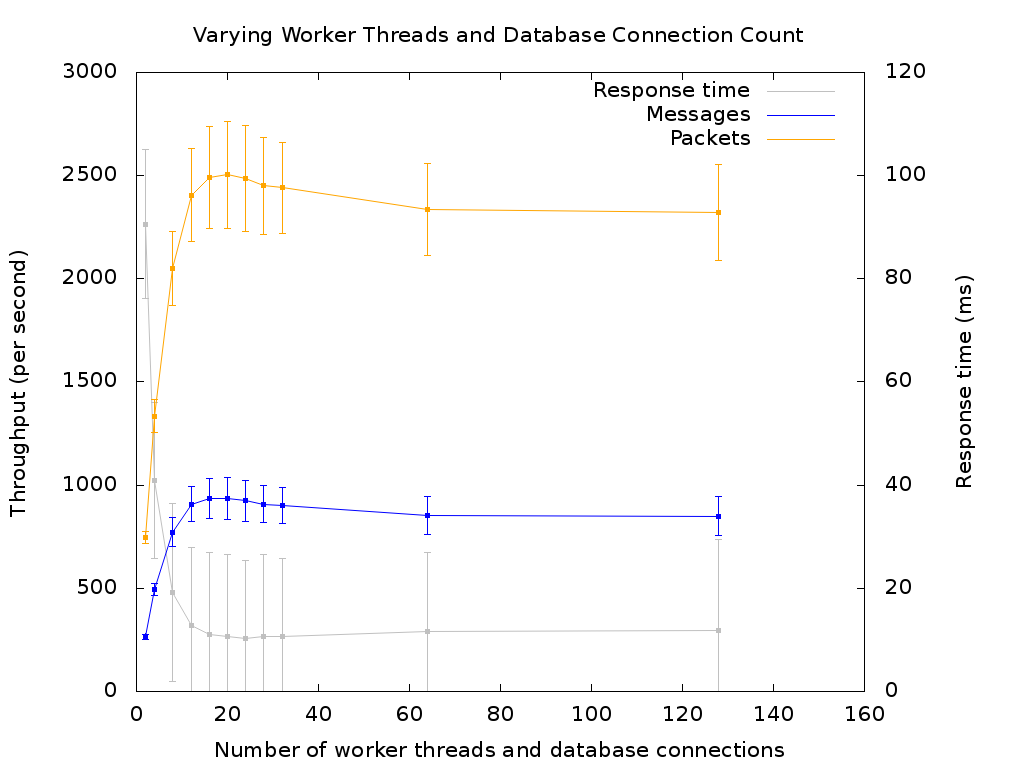
\includegraphics[width=0.9\textwidth]{graphs/db+worker}
            \caption{Varying number of worker threads and database connections}
            \label{fig:db+worker}
    \end{figure}
    
    \Cref{fig:db+worker} shows the comparison of both the response time and the
    throughput of the simulation and experiments varying the number of worker
    threads and database connections simultaneously.
    
    We see that the simulation roughly fits the measurements of the real
    \telesto{} system. The main differences are the extrema that are about $8
    \%$ off for the throughput and nearly trippled for the response time. Also
    they are reached at a later point than with the real world measurements.
    Over all, all simulated values start at higher values for the response
    time and lower values for the throughput but then follow approximately a
    similar slope like the comparison data.
    
    An other minor difference is, that the throughput does not show a clear and
    single maximum like in the measured values but stays constant after reaching
    the maximum value of $2792$ packets per second.
    
    \newpage
    
\subsection{Client Count}


    \begin{figure}[th]
        \centering
            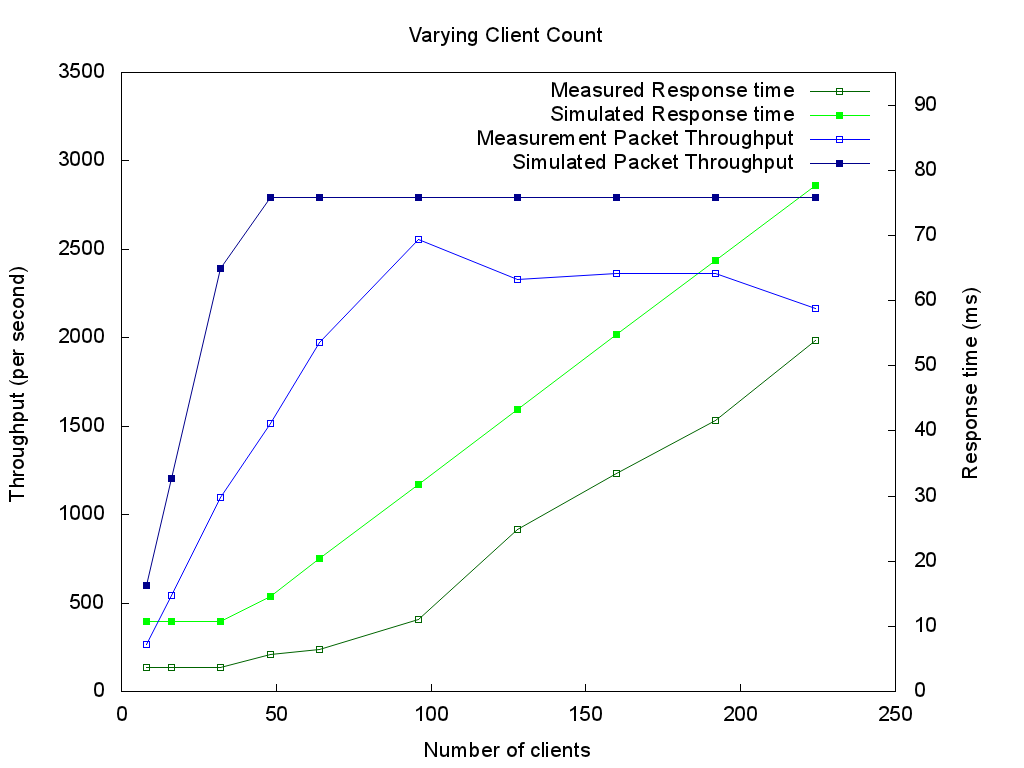
\includegraphics[width=0.9\textwidth]{graphs/client}
            \caption{Varying client count}
            \label{fig:clientCount}
    \end{figure}
    
    In \cref{fig:clientCount} we plotted the response time and throughput for
    \telesto{} when varying the number of clients and therefore jobs in the
    network.
    
    We can again say, that the curves take approximately the same development.
    The maximum of the throughput is about $9 \%$ off for the throughput while
    the response time has a very similar slope but is constantly off by about
    $20-25$ ms. Also we see, that the MVA model is limited in a way that it
    cannot simulate the descending throughput after a certain amount of clients
    are surpassed. (i.e. $100$ clients)
    
    Again the starting points are already not fitting the real values which
    itself produces a high offset.
    
    \newpage
    
\subsection{Client Retry Delay}
    
    
    \begin{figure}[th]
        \centering
            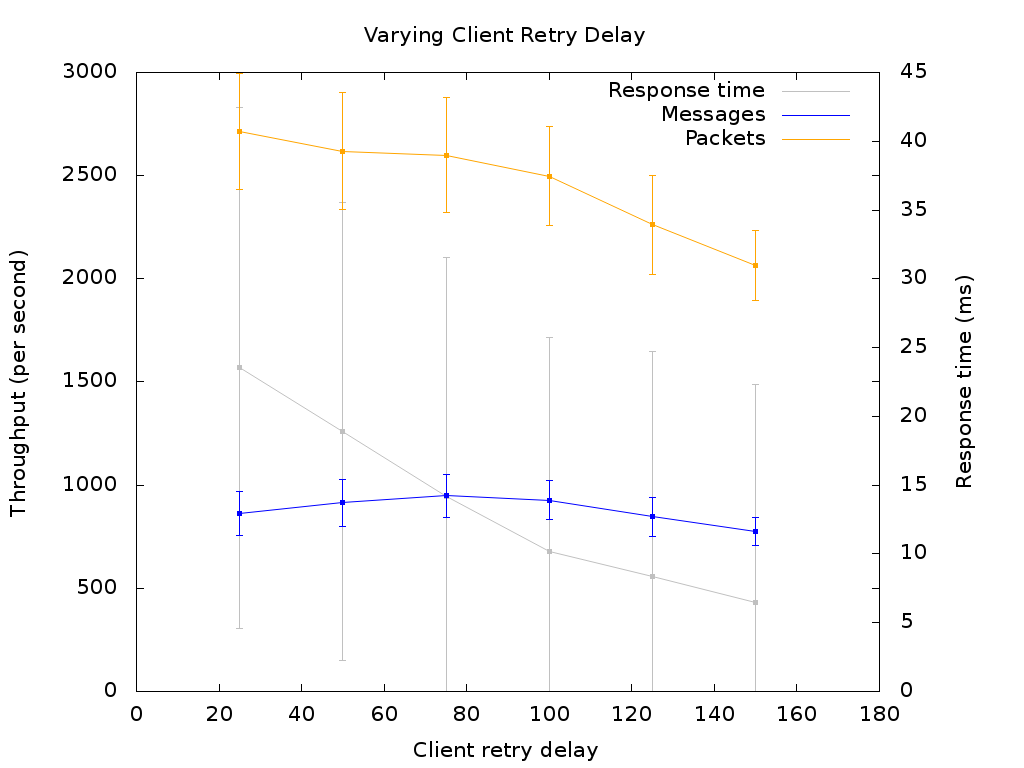
\includegraphics[width=0.9\textwidth]{graphs/client-delay}
            \caption{Varying client retry delay (i.e. think time)}
            \label{fig:retry-delay}
    \end{figure}

    Since the network think time is directly dependent on the client retry delay
    in \telesto, we also simulated this experiment with our MVA model. The
    results are shown in \cref{fig:retry-delay}.
    
    As presented in \cref{sc:parameters}, the client retry delay directly
    affects the think time of the modeled network. This can very nicely be seen
    in this comparison because we actually get very similar data for our
    simulation and the measurements from milestone 1. 
    
    Especially the retry delay in the interval of $75-100$ ms which leads to the
    best performance, produces very similar results with an offset of less than
    $7 \%$ and $3 \%$ for $75$ and $100$ ms respectively in throughput and less
    than $6 \%$ and $11 \%$ in response time.
    
    An other observation is that the measured response time continues to
    decrease with higher retry delay while the simulated one evens out at around
    $10.7$ ms. This is most likely because the probability of having to wait
    that long for a new message to be accessible is very low and doesn't behave
    in such a linear manner as it was modeled in the network model.
    
    \newpage

\subsection{Bottleneck}
    For bottleneck analysis we use the calculated utilization values from our
    MVA simulation. We used the standard configuration with $20$ worker threads
    and database connections, and $90$ clients which is the best performing
    configuration in our \telesto{} benchmarks in milestone 1.
    \Cref{tbl:utilization} shows the calculated data where we can clearly
    recognize that the database is as expected the bottleneck of the system.
    
     \begin{table}[ht]
        \centering
        
        \begin{adjustbox}{center}
            \rowcolors{1}{Gray}{white}
            \begin{tabular}{$l|^c}
                \rowcolor{DarkGray}
                \rowstyle{\bfseries}
                Center          & Utilitzation \\
                \hline
                
                Dispatcher      & 2.7 \% \\
                Middleware In   & 3.1 \% \\
                Database        & 100 \% \\  
                Middleware Out  & 4.8 \% \\
            \end{tabular}
        \end{adjustbox}
        \caption{Utilization of the load centers in the MVA simulation}
        \label{tbl:utilization}
    \end{table}
    
    
    

\section{Database}
    To get further information about how the database behaves during execution,
    we use a M/M/m queue model as described in \cite{jain2008art} and feed it
    with our measured values for the reference test of \telesto{} with $90$
    clients and $25$ database connections.
    
    We will do such an analysis only for the database part of \telesto{} since
    the middleware has such low utilization that it wouldn't really produce very
    interesting results. Our assumptions are that the middleware would have a
    very high probability for very low number of jobs in the queue, very low
    traffic intensity and practically no waiting time.

    In the following we state the formulas and calculations results directly as
    listed in Box 31.2 in \cite{jain2008art}. The calculations were done
    using a small python script that makes use of the {\tt
    decimal}\websource{Python
    Documentation:
    decimal Package}{http://docs.python.org/2/library/decimal.html}{December 20,
    2013} package in order to achieve very high precision with floating point numbers. A first try with a Java program using normal {\tt double}s yielded highly unstable results due to rounding errors and bad accuracy.

    \begin{align*}
        \text{Arrival rate}  & \qquad \lambda = 2498 \text{ jobs}\cdot s^{-1} \\
        \text{Service rate}  & \qquad \mu = 124.1 \text{ jobs} \cdot s^{-1} \\
        \text{Number of Servers}        & \qquad m       = 25   \\
        \text{Number of Jobs / Clients} & \qquad n       = 90
    \end{align*}

    While the value for $\lambda$ was directly extracted from the throughput
    measurements, $\mu$ was calculated using the mean service time for the
    database as already used for the MVA network simulation. The necessary
    calculations are shown below:

    \begin{align*}
        \mu = (0.008059s)^{-1} &= 124.1 \text{ jobs} \cdot s^{-1} \\
    \end{align*}
    
    \begin{figure}[th]
        \centering
            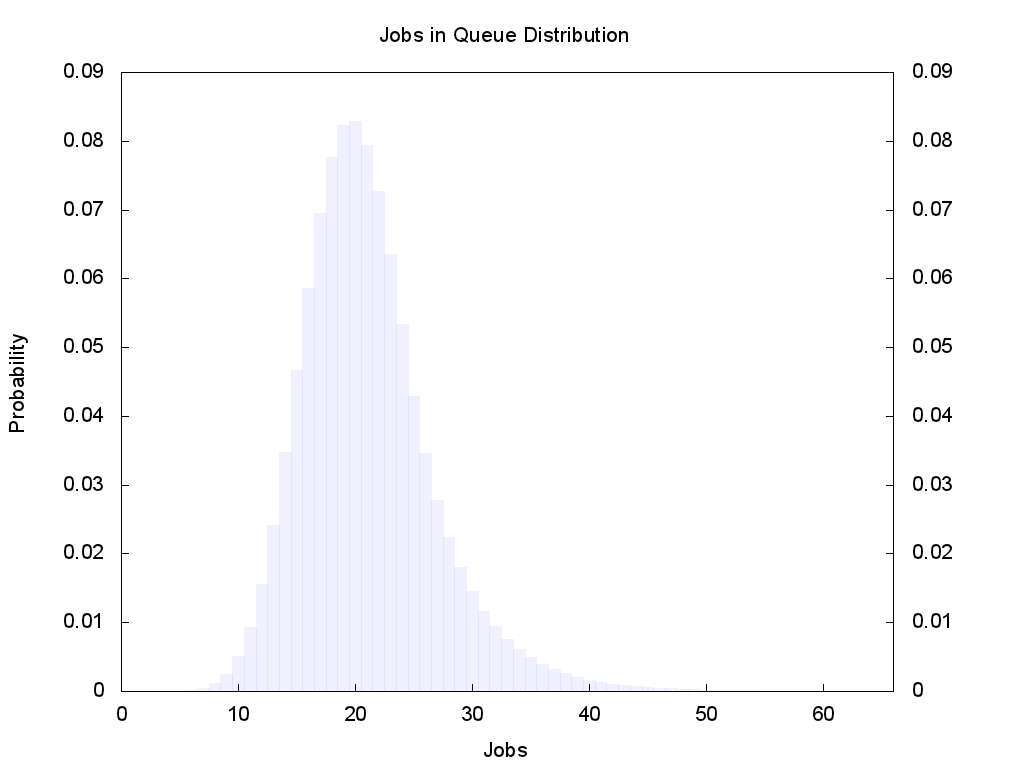
\includegraphics[width=0.9\textwidth]{graphs/histogram}
            \caption{Distribution of probabilities for a certian number of jobs
            in the system}
            \label{fig:jobs-in-queue-db}
    \end{figure}
    


\begin{description}
\item[Traffic Intensity:]
    \[
        \rho = \frac{\lambda}{m \cdot \lambda} = 0.805
    \]

\item[Probability of 0 jobs in Queue:]
\[
p_0 = \left[1 + \frac{(m*p)^m}{m! * (1-p)} + \sum_{n=1}^{m-1}
\frac{(m*p)^n}{n!}\right]^{-1} = 1.690 * 10^{-9}
\]

\item[Probability of n jobs in Queue:]
\[
p_n = \left\{
    \begin{array}{l l}
    p_0 * \frac{(m*p)^n}{n!} & n < m\\
    p_0 * \frac{p^n*m^m}{m!} & n \geq m
    \end{array} 
    \right.
\]

This formula yields \cref{fig:jobs-in-queue-db} which roughly fits a normal
distribution with highest probability for $21$ jobs with a value of
approximately $0.083 = 8.3 \%$.

\item[Probability of queuing:]
\[
\varrho = P(\geq m \text{ jobs}) = \frac{(m*\rho)^m}{m! * (1 - \rho)}*p_0 =
0.220 = 22.0 \%
\]

\item[Mean number of jobs in the system:]
\[
E[n] = m * \rho + \rho * \varrho /(1 - \rho) = 21.039
\]

\item[Variance of number of jobs in the system:]
\[
Var[n] = m * \rho + \rho * \varrho * \left[\frac{1 + \rho - \rho *
\varrho}{(1 - \rho)^2} + m\right] = 242.363
\]

\item[Mean number of jobs in the queue:]
\[
E[n_q] = \rho * \varrho / (1-\rho) = 0.910
\]

\item[Variance of number of jobs in the queue:]
\[
Var[n_q] = \rho * \varrho * \left[\frac{1 + \rho - \rho *
\varrho}{(1-\rho)^2}\right] = 7.605
\]

\item[Average utilization of each core (i.e. database connection):]
\[
U = \lambda/(m*\mu) = \rho = 0.805 = 80.5 \%
\]

\item[Mean response time:]
\[
E[r] = \frac{1}{\mu} * (1 + \frac{\varrho}{m * (1 - \rho)}) = 8.4 ms
\]

\item[Variance of the response time:]
\[
Var[r] = \frac{1}{\mu^2} * \left[1 + \frac{\varrho * (2 -
\varrho)}{m^2*(1 - \rho)^2}\right] = 0.066 ms = 66 \mu s
\]

\item[Mean waiting time:]
\[
E[w] = E[n_q]/\lambda = \varrho / [m * \mu * (1 - \rho)] = 0.364 ms
\]

\item[Variance of waiting time:]
\[
Var[w] = \varrho * (2 - \varrho)/[m^2 * \mu^2 * (1 - \rho)^2] = 1.072 \mu s
\]
This implies, that most jobs have to wait no more than about $1.3 ms$. Details
can be calculated using the $90-$ and $99-$percentile as below:

\item[90-Percentile of the waiting time:]
\[
\frac{E[w]}{\varrho} * ln(10 * \varrho) = 0.0013 s = 1.3 ms
\]

\item[99-Percentile of the waiting time:]
\[
\frac{E[w]}{\varrho} * ln(100 * \varrho) = 0.0051 s = 5.1 ms
\]
This means only $1 \%$ of all jobs have to wait more than $5.1$ ms and $10 \%$
more than $1.3$ ms.

\end{description}

As expected the utilization of the database with the selected input parameters
is quite high while the waiting time is still rather low. We expect this to
raise with increasing load. We also see a rather good correlation of the
calculated values with the real ones, given that we had very limited modeling
parameters.

\chapter{Conclusion}
	\label{ch:conclusion}
	
	Given that we only used the measured times of one execution of \telesto{} as
    input for the whole network model and for simulation of completely different
    configuration than those used during the reference measurement, the results
    were pretty good.
    
    The following sections will show some limits of the simulations and list
    some possible improvements.
	
\section{Limitations of MVA}
    First of all, it is very hard to model such a complex system with such a
    simple model that basically only takes runtimes of separate components as
    input. 
    
    Some factors like blocking, contention, mutual exclusion or
    non-exponential service times can simply not be modeled with the limited MVA
    model. 
    
    Then there is the problem of accurately selecting a $\mu$ function to
    model the load dependent behaviour of the database and the workers. In case
    of the workers, it is nearly irrelevant what is selected because they only
    make a very small part of the entire response time. But with the database we
    have a enormously complex software component that contains various
    optimizations, does many unpredictable memory reads and is just to complex
    as that if we could simply say it scales up to $25$ connections in parallel
    but with $10 \%$ overhead.
    
    We at this point assume, that most of the difference between our simulation
    data and the measured data is due to a too simplistic model of the database
    behaviour. However it is not the scope of this work to improve that model.
    
    In the usual case one would first do some very limited measurement with the
    system in order to have ground truth data for this model. There wouldn't be
    the whole set of real data to compare to and therefore we wouldn't be able
    to improve the model and change parameters in order to achieve a better fit.
    This is exactly why we didn't do this because this is not the goal of this
    simulation process.
    
    A second factor that impacts the correlation of our simulated data, is of
    course the think time of the network. Our estimation is very vague and holds
    only in a very small subset of the possible configurations. In order to
    improve the predictability of this parameter, it would have been better to
    only use \telesto{} tests with exactly one type of client and a guarantee of
    always getting a message back together with a constant waiting time after
    every response. This would lead to a predictable and balanced workload which
    is free from fluctuations.
 
    In the end we think the queuing network models as seen in
    \cite{jain2008art}, are quite useful for approximate simulation of systems
    that cannot be tested in real very easily. There is a big information source
    in modeling a system like that if it isn't already built completely or if
    further optimization options want to be explored without doing extensive
    real world testing.

\section{Multiple Middlewares}
    This report does not include any simulation of \telesto{} with multiple
    middlewares because it was relatively clear, that 
    \begin{enumerate}
        \item there wouldn't be any significant performance difference because
        the database is the bottleneck
        \item the model would get even more complicated with multiple
        middlewares.
    \end{enumerate}
    
    We therefore think that there is no real value in simulating this case and
    omitted it for this report.
    
% This displays the bibliography for all cited external documents. All references have to be defined in the file references.bib and can then be cited from within this document.
\bibliographystyle{splncs}
\bibliography{references}

% This creates an appendix chapter, comment if not needed.
%\appendix
%\chapter{Appendix Chapter}

%\section{Database Structure}

	
\end{document}